\section{Florestas Aleatórias}

Florestas Aleatórias (do inglês \textit{Random Forest}) é um algoritmo de aprendizado do tipo \textit{ensemble} cujo os meta-classificadores são Árvores de Decisão \cite{Quinlan:1986} treinadas com o método \textit{bagging}.
De acordo com \cite{breiman:2001} a definição formal do algoritmo Floresta Aleatória é dada por:

\begin{definition}\label{def:floresta}
Uma floresta aleatória é um classificador que consiste em uma coleção de classificadores de árvores de decisão ${h(x, \theta _k)}$, onde ${\theta _k}$ são as \textit{features} para o meta-classificador $k$ e, $x$ é o vetor de entrada.
\end{definition}

O algoritmo de Floresta Aleatória introduz um certo nível de aleatoriedade ao treinar os meta-classificadores; em vez de receberem o mesmo conjunto de dados, as árvores de decisão recebem um subconjunto diferente. Por exemplo, na figura \ref{fig:split_floresta} o \textit{dataset} original foi dividido em 2 subconjuntos de dados, os quais serão utilizados para treinar os algoritmos de árvore de decisão. Nota-se que as \textit{features} escolhidas não são as mesmas. Esse processo é importante, pois aumenta a capacidade de generalização do modelo de classificação.

\begin{figure}[h!]
    \centering
    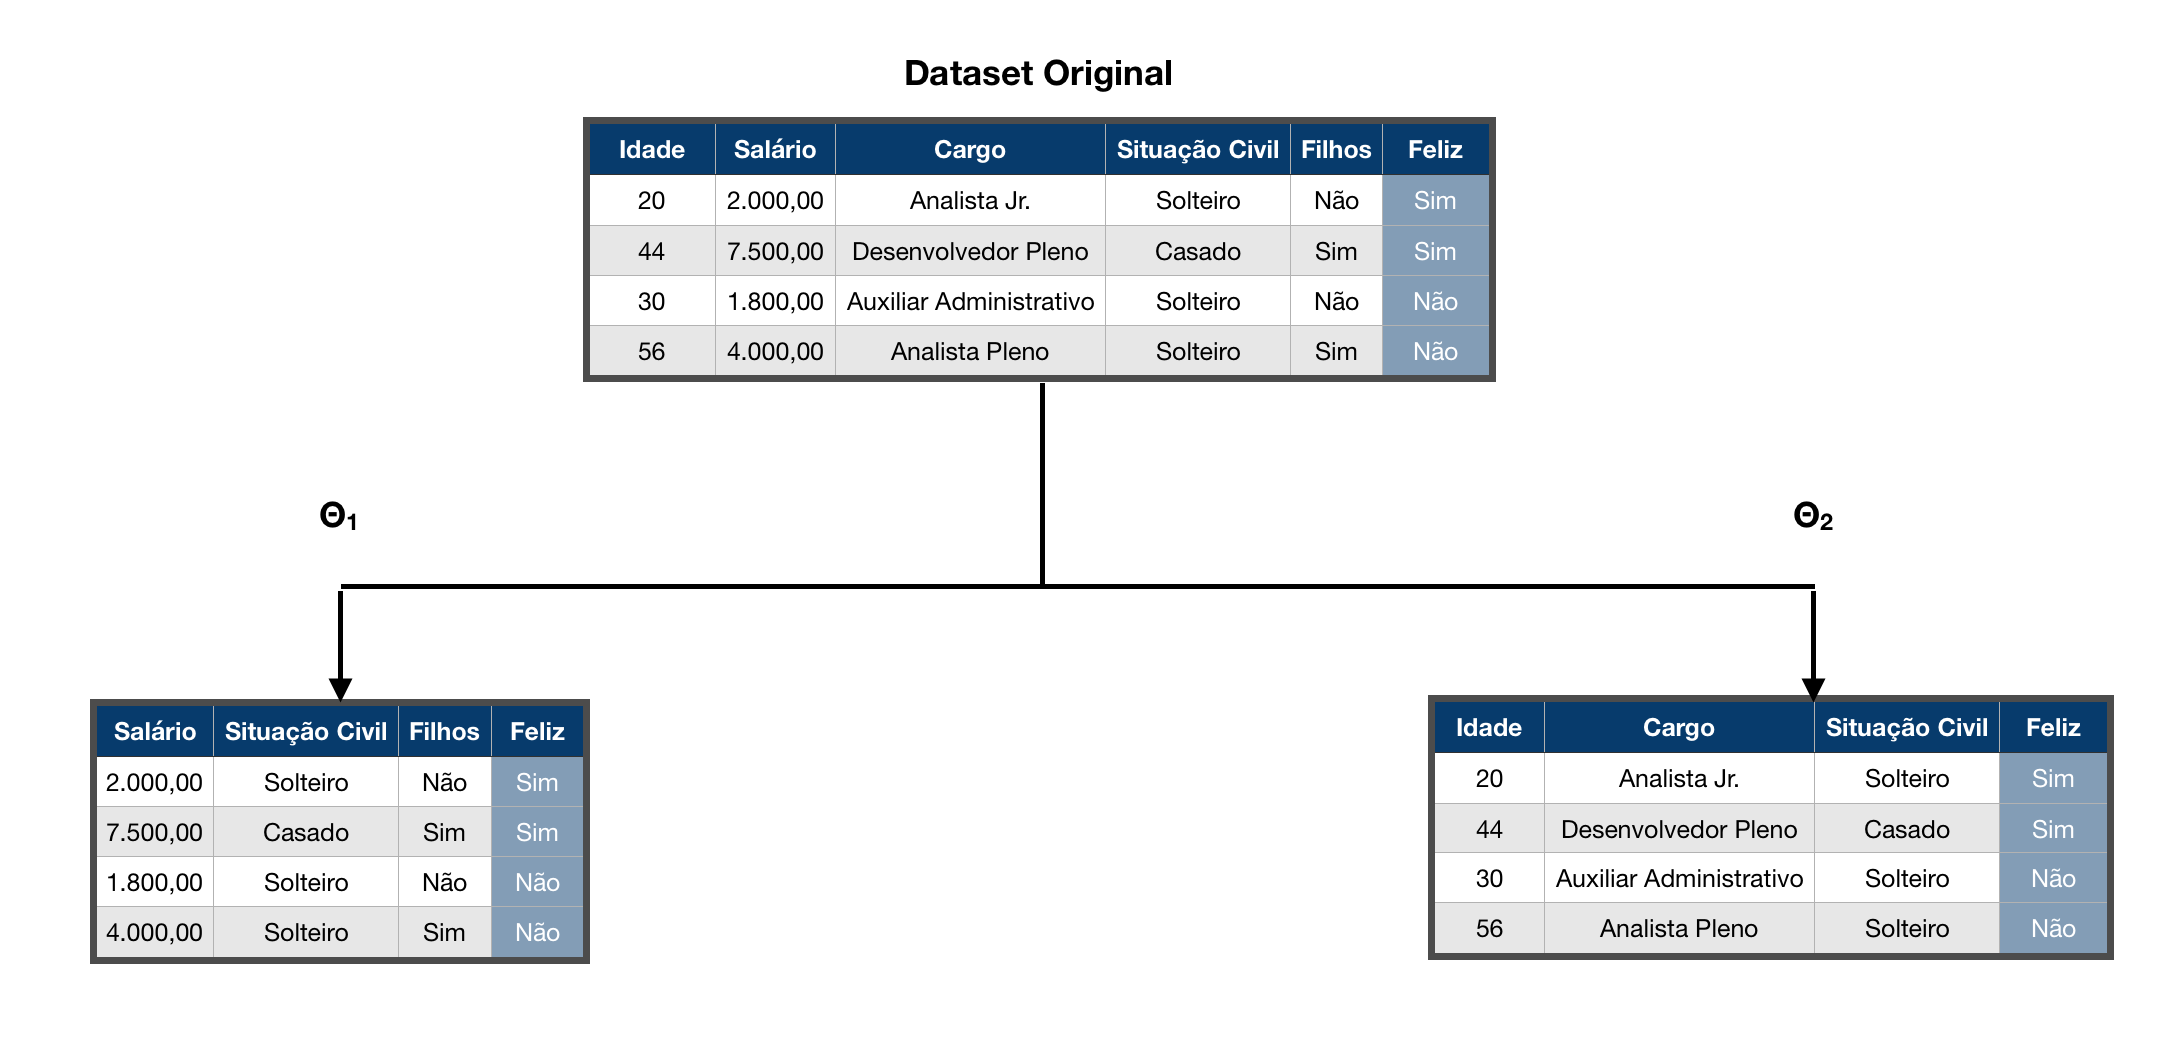
\includegraphics[scale=0.4]{Imagens/split_RandomForest.png}
    \caption{Exemplo de uma divisão randômica do \textit{dataset} original.}
    \label{fig:split_floresta}
\end{figure}

\subsection{A importância das features}
\label{sec:importancia_features}
Uma grande qualidade das florestas aleatórias é o fato de ser possível identificar as melhores \textit{features}, em outras palavras, é possível saber quais são os atributos mais importantes para predizer se um determinado registro irá pertencer a uma classe ou a outra. Se o modelo está sendo treinado para identificar uma doença de acordo com os sintomas, é possível descobrir quais são os sintomas que mais influenciam em um paciente possuir uma determinada doença.


\subsection{Vantagens e Desvantagens}
Um ponto positivo das Florestas Aleatórias é que esse tipo de algoritmo pode ser usado tanto para problemas de classificação quanto para problemas de regressão. 

Como foi dito na sessão \ref{sec:importancia_features}, é possível visualizar a importância de cada \textit{feature}, a fim de compreender melhor o comportamento dos dados e interpretar o modelo aprendido.

Um grande problema que aflige alguns algoritmos de aprendizado supervisionado é o \textit{overfitting}, isto ocorre quando um modelo aprende muito bem o conjunto de treino e sua capacidade de generalização fica comprometida por conta disso. Na maioria das vezes, esse problema não irá acontecer com o modelo de Floresta Aleatória.

A grande desvantagem do modelo de Floresta Aleatória fica por conta da sua performance quando há uma grande quantidade de árvores. Por um lado, quanto mais meta-classificadores melhor tende a ser a acurácia do modelo. Por outro lado, se há muitos meta-classificadores, a performance do algoritmo fica bastante comprometida.